\documentclass[11pt, oneside]{article}   	% use "amsart" instead of "article" for AMSLaTeX format
\usepackage{geometry}                		% See geometry.pdf to learn the layout options. There are lots.
\geometry{letterpaper}                   		% ... or a4paper or a5paper or ... 
%\geometry{landscape}                		% Activate for for rotated page geometry
%\usepackage[parfill]{parskip}    		% Activate to begin paragraphs with an empty line rather than an indent
\usepackage{graphicx}				% Use pdf, png, jpg, or eps� with pdflatex; use eps in DVI mode
								% TeX will automatically convert eps --> pdf in pdflatex		
\usepackage{amssymb}
\usepackage{amsmath}

\title{Fractional powers}
%\author{The Author}
\date{}							% Activate to display a given date or no date

\graphicspath{{/Users/telliott_admin/Dropbox/Tex/png/}}

\begin{document}

\maketitle
%\section{}
% \subsection*{R code}
% \begin{lstlisting}  \end{lstlisting}
% \begin{center} 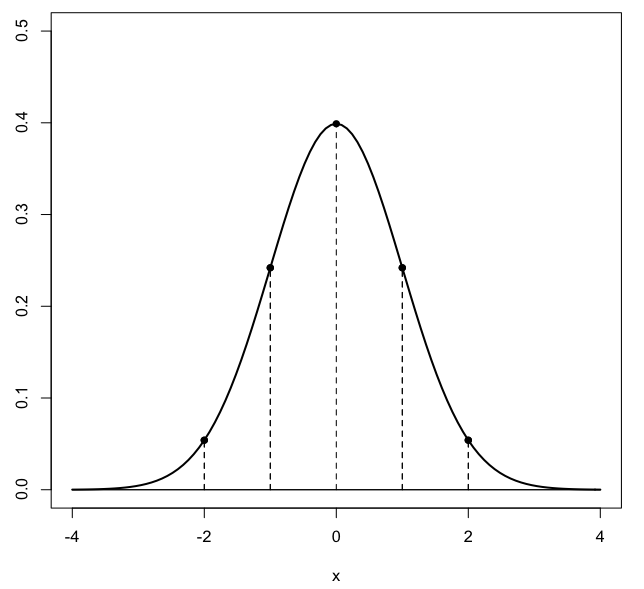
\includegraphics [scale=0.4] {gauss3.png} \end{center}
% \begin{bmatrix} a  &  b \\ c  &  d \end{bmatrix}
% \bigg |_

\large
In this short write-up we'll look at the difference quotient for simple roots of $x$
\[ \lim_{h \to 0} \frac{(x+h)^{1/n} - x^{1/n}}{h} \]

In the case of $\sqrt{x}$, we were able to clean up the numerator by multiplying by the conjugate
\[ \frac{\sqrt{x+h} - \sqrt{x}}{h} \ \  \frac{\sqrt{x+h} + \sqrt{x}}{\sqrt{x+h} + \sqrt{x}} \]
Giving
\[ \frac{x + h - x}{h \ \sqrt{x+h} + \sqrt{x}} \]
\[ \frac{1}{\sqrt{x+h} + \sqrt{x}} \]
\[ \frac{1}{2 \sqrt{x}} \]
in the limit as $h \to 0$.
\subsection*{4th root}
That approach does not work (at least not directly) for the cube root, but it does work for the fourth root

\[ [\ (x+h)^{1/4} - x^{1/4}\ ] \ [ \ (x+h)^{1/4} + x^{1/4}\ ] = [ \ (x+h)^{1/2} - x^{1/2}\ ] \]

We get back to the difference of square roots (in the numerator) and then just repeat, doing what we did above.  The denominator is finally
\[ \frac{1}{[(x+h)^{1/4} + x^{1/4}][(x+h)^{1/2} + x^{1/2}]} \]
and in the limit $\lim \to 0$
\[ \frac{1}{[\ 2x^{1/4}\ ] \ [ \ 2x^{1/2} \ ] } = \frac{1}{4} x^{-3/4} \]
which matches the power rule.  And it will work for any root that is a power of $1/2$.
\subsection*{Cube root}
A slight modification will do the same thing for the cube root.  The necessary factor is
\[ (a^{1/3} - b^{1/3})\ (a^{2/3} + a^{1/3}b^{1/3} + b^{2/3} ) \]
The inner terms cancel and we get 
\[ a - b \]
So we have
\[ [\ (x+h)^{1/3} - x^{1/3}\ ] \ [ \ (x+h)^{2/3} + (x+h)^{1/3}x^{1/3} + x^{2/3}\ ] = \ x + h - x \]
and after multiplying out the difference quotient (and subtracting $x$ and dividing by $h$) we will have
\[ \frac{1}{(x+h)^{2/3} - (x+h)^{1/3}x^{1/3} + x^{2/3}} \]
in the limit as $h \to 0$.
\[ \frac{1}{3x^{2/3}} = \frac{1}{3} x^{-2/3} \]
\subsection*{General method}
There are ways to solve this kind of equation for more complicated powers, and I will show one below.  However, there are better solutions to the general problem of $x^{m/n}$.  First, we can use Newton's expansion for the binomial, which has been proved for rational powers (though I don't think Newton actually proved it).  And there is another very elegant proof that uses implicit differentiation.  I have written about those elsewhere.
\subsection*{Cleaning up $x^{m/n}$}

The general method is essentially the same as for the cube root.  If we had

\[ (a^{m/n} - b^{m/n})(a^{n/m} + a^{m/n}b^{m/n} + b^{n/m}) \]
\[ = a +  a^{2m/n}b^{m/n} + a^{m/n}b^{n/m} - a^{n/m}b^{m/n} - a^{m/n}b^{2m/n} - b \]
which really looks like a mess!  But substitute $x+h$ for $a$ and $x$ for $b$ and what do we get?
Let's do the denominator first.  We will have
\[ h \ (a^{n/m} + a^{m/n}b^{m/n} + b^{n/m}) \]
\[ h \ [ \ (x+h)^{n/m} + (x+h)^{m/n}x^{m/n} + x^{n/m}\ ] \]
We'll be canceling the leading $h$, as you'll see in a second.  The numerator is really a bit of a mess, but we have
\[ = (x+h) +  (x+h)^{2m/n}x^{m/n} + (x+h)^{m/n}x^{n/m} - (x+h)^{n/m}x^{m/n} - (x+h)^{m/n}x^{2m/n} - x \]
Let's continue (boldly)
\[ = h +  (x+h)^{2m/n}x^{m/n} + (x+h)^{m/n}x^{n/m} - (x+h)^{n/m}x^{m/n} - (x+h)^{m/n}x^{2m/n} \]
Now, separate this into two parts.  Take that first $h$ over the denominator from above, which cancels to give
\[ \frac{1}{(x+h)^{n/m} + (x+h)^{m/n}x^{m/n} + x^{n/m}} \]
The second term, which is added to this one, has the same denominator (but without canceling $h$) and its numerator is what we had just before
\[ (x+h)^{2m/n}x^{m/n} + (x+h)^{m/n}x^{n/m} - (x+h)^{n/m}x^{m/n} - (x+h)^{m/n}x^{2m/n} \]
Now what will happen to this in the limit as $h \to 0$?  This becomes
\[ x^{2m/n}x^{m/n} + x^{m/n}x^{n/m} - x^{n/m}x^{m/n} - x^{m/n}x^{2m/n} \]
\[ x^{3m/n} + x - x - x^{3m/n} \]
This is just $0$, so the whole second term is $0$, and we are left with
\[ \frac{1}{x^{n/m} + x^{m/n}x^{m/n} + x^{n/m}} \]
\[ \frac{1}{x + x^{2n/m}} \]






\end{document}  